\section{Design} \label{sec:design}

%% See poetry_questions_full.tex for a four-column version
\begin{table}[t]
{\small
\def\arraystretch{1.1}
\begin{tabular}{p{1.8in}p{1in}}
\textbf{Question} & \textbf{Agent concerned} \\[.1cm]
\textbf{\emph{Word level}} & \\
What does this word mean? & WordNet expert \\
%%%%%%%%%%%%%%%%%%%%%%%%%%%%%%%%%%%%%%%%%%%%%%%%%%%%%%%%%%%%%%%%%%%%%%%%%%%%%%%%
Where does this word come from? & Provenance expert \\[.5cm]
%%%%%%%%%%%%%%%%%%%%%%%%%%%%%%%%%%%%%%%%%%%%%%%%%%%%%%%%%%%%%%%%%%%%%%%%%%%%%%%%
\textbf{\emph{Phrase level}} & \\
What is this line about? & Keywords expert \\[.5cm]
%%%%%%%%%%%%%%%%%%%%%%%%%%%%%%%%%%%%%%%%%%%%%%%%%%%%%%%%%%%%%%%%%%%%%%%%%%%%%%%%
\textbf{\emph{Line level}} & \\
What is the sentiment of this line? & Sentiment expert\\
Is this alliteration, rhyme, consonance, etc.~important? & Style expert \\[.5cm]
%%%%%%%%%%%%%%%%%%%%%%%%%%%%%%%%%%%%%%%%%%%%%%%%%%%%%%%%%%%%%%%%%%%%%%%%%%%%%%%%
\textbf{\emph{Poem level}} & \\
How many rhymes are in the poem? & Rhymes expert \\
How well does the poem's metrical structure flow? & Rhythm expert \\
How repetitive is the poem? & Repetition expert
\end{tabular}
}
\caption{Questions we could implement using various computational agents\label{tab:questions_for_computational_agents}}
\end{table}

\subsection{Questions to ask when reading poems}

Table \ref{tab:questions_for_computational_agents} contains a list of
questions that could be addressed, in a programmatic manner, to
analyse an individual poem.  These questions, coming from a computer
poetry perspective, do not make the same assumptions about linguistic
understanding or embodied experience that apply to human poets.  It is
worthwhile to compare this list with a list of questions that a
reasonably sophisticated poetry reader might ask about poems (Table
\ref{tab:questions_for_human_readers}).  The difference between these
two frames of reference is most instructive.

In the approach to ``sophisticated'' reading considered here, we focus
on the process-oriented question: ``What does the poem tell us about
how it was made?''  This can be studied through the lens of the
follow-up question ``What are the aspects of the poem and how are they
present to the reader?''

%% See poetry_questions_full.tex for a narrative treatment of these questions

\begin{mdframed}
\textbf{I've compressed this down a lot.  Add some references and
  expand this a bit.  Our old notes may be useful.}

Among the several aspects that may be present in the poem are
register(s); addressee(s); position(s); the changing awareness of the
reader; character(s); image(s); functions, mechanics, and paradigms;
problems, discomforts, and dis-easements; apparent versus
substantiated truths; overlapping scenarios; chronology of reading and
chronological references; lexical choices that carry a deeper semantic
meaning; allusive effects; and manifest uncertainty in the poem's
construction.
\end{mdframed}

\begin{table}
{\small
\def\arraystretch{1.2}
\begin{tabular}{p{1.8in}p{1.1in}}
\textbf{Question} & \textbf{Examples} \\[.1cm]
What is are the register(s) of the poem? & cliched, instructive, imperative\\
Who is addressed? & friend, rival, lover, confidante, pupil\\
What position(s) are present in the poem? & pleading, remonstrating, ephemeral\\
What becomes of the reader whilst reading the poem? & alienated, perplexed, amused\\
Who are the characters in the poem? & ``the falconer'', ``you'', narrator, ``two men'' \\
What is the role of image(s) in the poem? & ``the sea'', ``a bicycle''; multiple meanings\\
What functions, mechanics, and paradigms are present for the reader to engage with? & communication, subverted cliche\\
What problems, discomforts, or dis-easements are invoked in the poem? & terror, self-loathing, rejection, desire \\
How do these evolve? & E.g. an image may start to take over from a register \\
What \emph{is} in the world of the poem as compared with what you only think is? & ``Surely'', ``must''; sacred vs mundane; perspectival vs surreal \\
What are the overlaps, transitions, implicit dialogues? & ``twinned'' lines/ideas, juxtaposed parts of the poem\\
What role does the chronology of reading play, versus references to chronology and chronological positions within the poem? & flagged development, evolution, movement, stasis\\
How are lexical categories used? & flimsy adverbs, solid nouns, thudding adjectives\\
Are there discernible allusive effects? & illustrating the literary apprenticeship of the author (or reader)\\
How does Keats' idea of negative capability feature in the composition -- ``that is when man is capable of being in uncertainties''? & we must worry about overconfidence, over-determined lines\\
\end{tabular}
}

\caption{Questions that we actually ask when reading a poem\label{tab:questions_for_human_readers}}
\end{table}

One of the striking things about this list is that it does not easily
divide itself into ``levels'' in the same way as the items in Table
\ref{tab:questions_for_computational_agents} do.  For instance, even
though lexical effects clearly have to do with an analysis taking
place at the ``word level'' the task that a given selection of words
performs is typically global; that is, it is meaningful at the ``poem
level.''  The questions in Table \ref{tab:questions_for_human_readers}
may themselves be divided into registers and positions.  The process
of reading a poem is also a process of \emph{poiesis}.  Each of the
examples listed in the right-hand column of this table (and a plethora
that are not listed) plays a role in the ``society of mind'' of a
reader, analogous to the agents in Table
\ref{tab:questions_for_computational_agents}.

\subsection{Bridges between `theory' and `practice'}

There are things we can actually point to in poems, and matching
concepts in aesthetic philosophy.  Furthermore, we can actually
approach this scientifically.  The computational approach to poetry is
one way to build the practice/theory bridge.  In particular, our
\emph{ansatz} is that the workshop could serve as a way to deepen an
understanding of a poem's semantics!

There are certain prerequisites.  In addition to the presentation of
written work, an underlying situation is assumed, one that is shared
(with respect to differing points of view) by the poet and the critic
(see Figure \ref{fig:cycles}).  The poet and critic are assumed to
have relatively stable, enduring but evolving, identities -- so that
it would be possible at a given juncture for either one to consider
the question ``Who am \emph{I}?''  and ``Who are \emph{you}?''
\cite[p. 251]{bakhtin1984problems}.

To begin with, in response to a given computer-generated poem:

{\itshape
\begin{verse}
%Demon dog\\[\baselineskip]
%
Oh dog the mysterious demon\\
Why do you feel startle of attention?\\
Oh demon the lonely encounter\\
ghostly elusive ruler\\
Oh encounter the horrible glimpse\\
helpless introspective consciousness\\
\end{verse}
}

A human critic might offer the following feedback:

\begin{quotation}
~\vspace{-1\baselineskip}
\begin{enumerate}
\item The use of the word \emph{mysterious} in the first line has no
  resolution, real or attempted, or quest to find one.
%
\item The use of the word \emph{attention} is not being interrogated
  or acknowledged for its importance.  Its qualifying word is
  \emph{startle}, used here as an adjective; acknowledging the fact
  that the attention is noted but not yet part of the transformative
  of the poem.
%
\item This is repeated in the next references to the aesthetic
  experience as a \emph{lonely encounter} and an \emph{exclusive
    ruler}, which is then qualified as \emph{a horrible glimpse}.
%
\item So reference to the contact made between the poem and its own
  event are made through the words \emph{demon}, \emph{encounter} and
  \emph{consciousness} and all of these are qualified in negative
  terms.
%
\item This poem does not welcome the intimacy of bringing anything to
  aesthetic consciousness so that it might be expressed. Why do I say
  that? Because the words are generalised and \emph{horribly}
  imprecise.
%
\item The really interesting thing about it is its own apparent
  understanding that this is so.  Look at the words \emph{mysterious},
  \emph{feel} \emph{lonely}, \emph{elusive}, \emph{horrible},
  \emph{glimpse}, \emph{helpless}, \emph{introspective},
  \emph{conscious}. They are unspecific -- nothing has been explored
  as the poem moves toward a better understanding of these ideas. They
  describe but they do not illuminate by becoming anything else. They
  all associate exploration with fear and isolation and this is
  (paradoxically) quite an interesting acknowledgment of the poem’s
  refusal to go anywhere i.e become a thing transformed by a creative
  process.
\end{enumerate}
\end{quotation}

Each of these comments is \emph{dual-voiced} in the sense that the
critic is relaying the poet's speech with a new emphasis.  Each such
statement is one side of a micro-dialogue
\cite[p. 73]{bakhtin1984problems}.  The challenge is, of course, to
bring the observations into the awareness of the poet, across the
``silicon divide.''  From the programmer's standpoint, this involves
massaging each of the observations into a language that the computer
can understand -- the most obvious candidate being the programming
language the computer used to generate the poem.  But care should be
taken not to just blythely program the computer with more rules, but
rather to give attention to the process of learning new rules
contextually.

Rather more briefly, let us consider a reversal of roles, and put the
computer in the position of critic, looking at a passage from an
historical piece of poetry.  We have selected one that might have --
but in fact did not -- serve as a model for the poem generated above.

{\itshape
\begin{verse}
I'm truly sorry man's dominion\\
Has broken Nature's social union,\\
An' justifies that ill opinion\\
Which makes thee startle\\
At me, thy poor, earth born companion\\
An' fellow mortal!\\
\end{verse}
}

Naturally, the first problem is for the computer to \emph{read} the
poem.  There are various possible approaches to this problem.  One of
the approaches that is most appealing from our point of view is the
automatic generation of a semantic network from the input text
\cite{harrington2007asknet}.  This, again, could be enhanced by
additional meanings that are not just factual, say, but aesthetic
(drawing on the notions informing Table
\ref{tab:questions_for_human_readers}).

We do not propose that either of these programming tasks is entirely
easy, but both are entirely feasible.


\begin{figure}
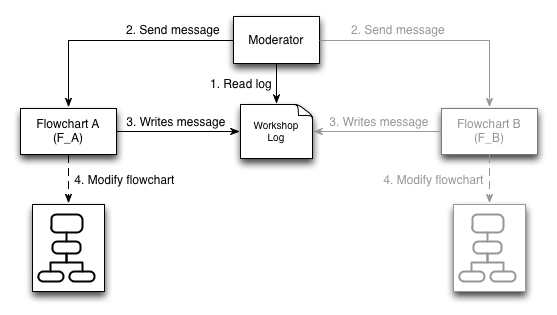
\includegraphics[width=\columnwidth,trim = 0mm 0mm 2mm 0mm,clip=true]{figures/workshop-diagram}
\caption{Schematic design for a workshop built in the FloWr system}
\end{figure}

\subsection{Prototyping a workshop in FloWr}
Development plan (Christian):
\begin{itemize}
	\item Define workshop, including product properties, e.g. variety, innovation, etc. Alternatively, refer to prior definition earlier in the paper and point out benefits again.
	\item Introduce different roles in a workshop: master, working student, criticising student (anything else?). These roles can be combined into more complex ones. 
	\item Introduce tasks they perform: introducing and demonstrating new tools, using tools to generate, analyse to improve creation, etc.
	\item Show the demon dog flowchart as part of the FloWr system, and highlight which roles the different parts represent, and which tasks are present.
	\begin{itemize}
		\item A flowchart could be identified as a student that both creates and asseses (fitness functions) at the same time.
		\item The script/moderator could be identified as the master who guides the student, tells it what to do in which way.
		\item The set of all process nodes can be understood as a toolbox the master can access, to hand tools to the student.
	\end{itemize}
	\item Show what's missing to fulfill the prior definition of a workshop
	\begin{itemize}
		\item Multiple students that collaborate and help improving each other's creations.
		\item Master as mediator between two students, asking one student what tools it uses, and telling the other to adapt them.
		\item The moderator can introduce new tools to the workshop.
		\item Students must be able to notice at one step of the creation process (e.g. while using one tool), that the usage of a prior tool could be improved. They could then either first finish or rewind.
		\item Allow for more than one agent. Allow for more than one agent to work at a time.
	\end{itemize}
\item Show which features are required to realize that:
	\begin{itemize}
	\item Understanding the workshop as a hierachical multi-agent system, where the master is at the top and the students are at the bottom of the hierarchy. 
	\item Simplification by separating flowcharts that create and assess from those which only assess. 
	\item Thus introducing external assesment.
	\item Thus communication between flowcharts required.
	\item Enable an agent (more general, e.g. a student) to explain what tools it is using, in which order, and which parts of the output they affect.
	\item Allow other agents to improve their flowchart by means of this information, e.g. add a particular tool in a particular step.
	\item Enable master as mediator.
	\item Allow master to map observations of poems into new tools, that are made available to the workshop.
	\item Allow communication between process nodes, i.e. tools: E.g. assessment in rhyming node shows that too few words/sentences available for good results. Thus necessary to fetch more/different sentences in a prior step. Problem: agency when using the term "tool" - separates assessment by the agent from using the tool for creation.
	\item Introduce parallelisation, to allow multiple agents to work at the same time.
	\end{itemize}
\item Open questions:
\begin{itemize}
	\item Decision making: It's probably more important to answer how decisions are made to adapt another tool, etc., than stating where they're made. E.g. decision making by means of a fitness function of the current artefact, by means of curiosity, etc.
	\item Add more implementation suggestions
	\item Would it be better to focus on one new aspect of the workshop, and leave the others out? E.g. add master who can introduce new tools, or introduce multiple students that can communicate. One paper might be not enough to get from current FloWr to a full-fledged workshop.
\end{itemize}
\end{itemize}


\begin{mdframed}
\textbf{What's the development plan look like?  Should we show the
  flowchart for the ``demon dog'' poem as a very early prototype and
  concrete example to critique?  We could illustrate -- in principle
  -- how it would be improved in a workshop.}

We'll need to discuss the different levels of the design.  E.g.

Moderator.  

Flowchart A: ``I do this'' (service advertising what facilities it has available: if we can swap them in and out, we could do some kind of A/B test to check whether swapping in a different node actually improves the result according to some critic or other).

Flowchart B: ``I would like to be able to do that too.''
Temporality. More feedback from critical agents.  Learn and adapt the script.

Where is the decision made to modify (e.g. only by the Moderator, or at the level of individual flowcharts, or nodes, etc.?)

This is relevant to the issue of ``parallel solutions''.  At the level of some downstream process: How do we decide which of the parallel solutions to pick and carry ahead to the next step?  Do we give feedback to the previous step in the process?

If we are allowed to take multiple different paths, not just parallel copies of the same process, where is the decision made as to which path to take?

Central control
Distributed control
Autonomous
Global wiring

Critic: ``This `Twitter' node is not good.''

Follow the idea of the prepared mind, add any problem that is noticed to a list of ``problems to solve.''  Again, the log of suggestions/outstanding problems could exist at different levels/timescales.  (NB. And a similar approach can apply for ``questions'' as well as ``problems.''  This ``log'' doesn't just have to be a list, it could also be a frame or flowchart etc.)

Protocol:

flowchart to flowchart?

Do we also need some modification for node-to-node communication?
Alternatively, are we going to follow Christian's suggestion and merge flowcharts and nodes into one kind of entity?

Also, do we need an overall ``protocol'' for the Workshop demo
application, different from the more general communication protocol
that is used?

There will be three different type of messages: questions, answers and
suggestions.

Questions can be about sources of information; e.g. files, online
articles, input from another node, etc., about elements of poems;
e.g. similes, rhymes, keywords, sentiment, etc.; about specific
details; e.g. count, purpose, etc. Answers would be associated to
previous questions, and suggestions are changes proposed by one system
to the other.

Commentary is needed in order to enable the dialogue between
flowcharts. Each node in FloWr has two main components, a set of input
parameters and a set of output variables.  Parameters can either be
sources of information; e.g. the Guardian newspaper, or conditions;
e.g. range of dates. Variables are outputs of different types.  A
commentary would be added to each of them in order to facilitate
communication between flowcharts and nodes. This will enable the
dialogue between the participants in the workshop; i.e. ask and answer
questions, as well as it will allow to identify where to apply
suggestions for new versions of a flowchart as suggested in a workshop
session. The proposed commentary is presented in an Appendix.

%% These were some potential criticisms that seem mostly directed at this level

Do we consider e.g. genetic algorithms present (i.e. generate) several
options and allow the downstream nodes to comment on each one high
level feedback (on the whole generated poem) and micro-feedback (at
the level of individual nodes)

Atomic nodes vs composite nodes (flowcharts).  Can we just forget
about what level we are at?  Node or flowchart -- and use a recursive
approach that can be applied to atomic or composite nodes?
(Christian’s diagram of the two different kinds of communication --
between flowcharts or between nodes -- reduce to one kind of
communication if we take the recursion approach.  Similarly,
reification then becomes possible.  In itself this isn’t a huge
technical advance, but it might allow us to deal with examples of
``morphogenesis'', which is interesting.  E.g. grow until I have 100
process nodes and then stop. That said, ``reification'' is a bit
frowned upon -- but provenance is always a good thing.)
\end{mdframed}



%%% Local Variables: 
%%% mode: latex
%%% TeX-master: "mathsICCC"
%%% End: 
